\chapter{Grammatiche e Linguaggi Context-free}
In informatica i linguaggi formali sono di vitale importanza.
Essi sono utilizzati come rappresentazione formale di problemi di decisione e l’eventuale soluzione algoritmica a tali problemi si traduce nell’esistenza o meno di modelli di computazione per il riconoscimento delle stringhe di un linguaggio.
La teoria sviluppata è uno degli esempi più evidenti di come lo studio di un argomento teorico, e la comprensione delle proprietà formali dei suoi elementi abbia permesso lo sviluppo di tecniche automatiche per risolvere efficientemente compiti che richiedevano tempi e risorse non banali.

L’esempio più significativo è quello della costruzione di quelle parti dei compilatori che acquisiscono i programmi degli utenti, ne verificano la correttezza “lessicale” e “sintattica” e ne trasformano la rappresentazione in modo da agevolare i passi successivi di analisi, ottimizzazione e generazione del codice da eseguire.
Questi analizzatori lessicali e analizzatori sintattici, come vengono chiamati, sono disponibili fin dalla fine degli anni ’70 e in brevissimo tempo realizzano quello che in precedenza ne richiedeva molto di più.
Una serie di risultati teorici ha reso possibile costruire programmi che “programmano”.

Esamineremo i linguaggi da due punti di vista complementari, basati sull’approccio riconoscitivo e su quello generativo.
In particolare, nell’approccio riconoscitivo studieremo procedure, sotto forma di “automi,” che definiscono un linguaggio attraverso “l’accettazione” delle stringhe che lo costituiscono.
Seguendo l’approccio generativo invece, si definiscono meccanismi di calcolo che sono sistemi di riscrittura particolari e sono chiamati “grammatiche,” attraverso le quali si possono ottenere, appunto generandole, le stringhe del linguaggio in questione.
Partiremo da grammatiche abbastanza semplici ma che giocano un ruolo importante nella sintassi dei linguaggi di programmazione, le grammatiche context-free.

\subsubsection{Un esempio informale: parole palindrome}
Una parola e palindroma se letta da sinistra a destra o da destra a sinistra dà luogo alla stessa sequenza.
Quindi una parola $w \in \Sigma^{*}$ è palindroma se e solo se $w=w^{R}$.
Esempi: alla, otto, abba, amima.

Definizione ricorsiva delle parole palindrome sull'alfabeto $\{a, b\}:$

PASSO BASE: $a, b$ e $\epsilon$ sono parole palindrome.

PASSO RICORSIVO: Se $x$ è una parola palindroma allora anche $a x a$ e $b x b$ sono parole palindrome.

Esempio: $a b b a$ è palindroma

\vspace{5mm}

(PASSO BASE) $\epsilon$ è una parola palindroma

(PASSO RICORSIVO) $b \epsilon b=b b$ è una parola palindroma

(PASSO RICORSIVO) abba è una parola palindroma.

\subsubsection{Un esempio informale: dalla definizione ricorsiva alla grammatica}
Le regole che definiscono le parole palindrome sull'alfabeto $\{a, b\}$ nella notazione delle grammatiche libere dal contesto:

(1) $S \rightarrow \epsilon$

(2) $S \rightarrow a$

(3) $S \rightarrow b$

(4) $S \rightarrow a S a$

(5) $S \rightarrow b S b$

\subsubsection{Definizione di una grammatica context-free}

Una grammatica libera dal contesto (o grammatica context-free, o CFG o grammatica) G, è una quadrupla
$G=(V, T, P, S)$
dove:
\begin{itemize}
    \item V: Insieme finito di variabili (dette anche non terminali o categorie sintattiche). Ogni variabile rappresenta un linguaggio.
    \item $T$ : Insieme finito di simboli terminali (o alfabeto dei terminali). È l'alfabeto delle parole del linguaggio da definire. $T \cap V=\emptyset$.
    \item P: Insieme finito delle produzioni (o regole) che rappresentano la definizione ricorsiva di un linguaggio.
    \item S: Una variabile, detta simbolo iniziale (o start symbol), che rappresenta il linguaggio definito dalla grammatica. Altre eventuali variabili rappresentano insiemi ausiliari di stringhe che contribuiscono a definire il linguaggio del simbolo iniziale.
\end{itemize}

Ogni produzione consiste di tre parti.
\begin{enumerate}
    \item Una variabile (definita parzialmente dalla produzione), detta anche testa della produzione
    \item Il simbolo di produzione $\rightarrow$
    \item Una stringa di zero o piu terminali e variabili, detta anche corpo della produzione.
\end{enumerate}
La grammatica $G_{p a l}$ per le parole palindrome sull'alfabeto $\{a, b\}$ è rappresentata da\footnote{Nota. Nelle espressioni regolari, alcuni autori usano + per denotare l’operatore $\cup$.}
$$
G_{p a l}=(\{S\},\{a, b\}, P, S)
$$
dove
$$
P=\{S \rightarrow \epsilon, S \rightarrow a, S \rightarrow b, S \rightarrow a S a, S \rightarrow b S b\}
$$

\subsubsection{Esempio - Espressioni}
Una grammatica per le espressioni aritmetiche in un linguaggio di programmazione.
Semplifichiamo: per gli identificatori usiamo solo le lettere a e $b$ e le cifre 0 e 1 .
Un identificatore è un elemento dell'espressione regolare
$$
(a+b)(a+b+0+1)^{*}
$$
Due variabili:
\begin{itemize}
    \item E per le espressioni,
    \item I per gli identificatori
\end{itemize}
Dobbiamo fare riferimento a una definizione ricorsiva degli elementi di
$$
(a+b)(a+b+0+1)^{*}
$$
Le produzioni:
\begin{enumerate}
    \item $E \rightarrow 1$
    \item $E \rightarrow E+E$
    \item $E \rightarrow E * E$
    \item $E \rightarrow(E)$
\end{enumerate}

\vspace{5mm}

\begin{enumerate}
    \item $I \rightarrow a$
    \item $I \rightarrow b$
    \item $I \rightarrow Ia$
    \item $I \rightarrow Ib$
    \item $I \rightarrow I0$
    \item $I \rightarrow I1$
\end{enumerate}

Una CFG per espressioni aritmetiche:
$$
G_{E}=(\{E, I\}, T, P, E)
$$
dove
$$
T=\{+, *,(,), a, b, 0,1\}
$$
 $P=\{E \rightarrow I, E \rightarrow E+E, E \rightarrow E * E, E \rightarrow(E), I \rightarrow a,$, $I \rightarrow b, I \rightarrow l a, I \rightarrow I b, I \rightarrow I 0, I \rightarrow I 1\}$
 
\subsubsection{Notazione compatta per le produzioni}
Invece di
$$
A \rightarrow \alpha_{1}, A \rightarrow \alpha_{2}, \ldots, A \rightarrow \alpha_{n}
$$
possiamo scrivere
$$
A \rightarrow \alpha_{1}\left|\alpha_{2}\right| \ldots \mid \alpha_{n}
$$
Esempio. In $G_{p a l}=(\{S\},\{a, b\}, P, S)$
$$
P=\{S \rightarrow \epsilon|a| b|a S a| b S b\}
$$

\subsubsection{Derivazione}
Applichiamo le produzioni di una grammatica per dedurre che alcune parole sono nel linguaggio di una variabile.
La deduzione può seguire due strade:
\begin{enumerate}
    \item usare l'inferenza ricorsiva (dal corpo alla testa)
    \item usare la derivazione (dalla testa al corpo)
\end{enumerate}
Non tratteremo l'inferenza ricorsiva.

\subsubsection{Derivazione diretta}
Sia $G=(V, T, P, S)$ una grammatica context-free.
Sia $\alpha A \beta \in(V \cup T)^{*}, \operatorname{con} A \in V e \alpha, \beta \in(V \cup T)^{*}$,
Sia $A \rightarrow \gamma \in P$.


Allora diremo che
$\alpha A \beta$ deriva (direttamente)  $\alpha \gamma \beta$
e scriveremo
$$\alpha A \beta \xRightarrow[G]{} \alpha \gamma \beta$$  

o, se $G$ è chiara dal contesto, semplicemente
$\alpha A \beta \Rightarrow \alpha \gamma \beta$

\vspace{5mm}

Quindi $\alpha A \beta$ deriva direttamente $\alpha \gamma \beta$ se $A \rightarrow \gamma \in P$, con $\alpha, \beta$ stringhe di variabili e terminali.
Nella grammatica definita dalle regole $S \rightarrow \epsilon|a| b|a S a| b S b$
\begin{itemize}
    \item $S \Rightarrow$ aSa, con $\alpha=\beta=\epsilon$
    \item aaSaa $\Rightarrow$ aabSbaa, con $\alpha=\beta=a a$
    \item $a b S b a \Rightarrow a b b a, \operatorname{con} \alpha=a b, \beta=b a$
\end{itemize}
$\alpha A \beta$ deriva direttamente $\alpha \gamma \beta$ se $A \rightarrow \gamma \in P$, con $\alpha, \beta$ stringhe di variabili e terminali.
Nella grammatica definita dalle regole $E \rightarrow E+E|E * E|(E) \mid I$,
$I\rightarrow a| b|Ia| Ib| I0 | I1$
\begin{itemize}
    \item $ E \Rightarrow I, \operatorname{con} \alpha=\beta=\epsilon$
    \item $ E+E \Rightarrow E+E * E, \operatorname{con} \alpha=E+, \beta=\epsilon$
    \item $ a *(E+E) \Rightarrow a *(I+E), \operatorname{con} \alpha=a *(, \beta=+E)$
\end{itemize}

Nella grammatica definita dalle regole $S \rightarrow \epsilon|a| b|a S a| b S b$ abbiamo
$$
S \Rightarrow a S a, a S a \Rightarrow a b S b a, a b S b a \Rightarrow a b b a
$$
Definiremo una nuova operazione:
$$
S \xRightarrow[]{*} a b b a
$$

\subsubsection{Derivazione}
Estendiamo la relazione $\Rightarrow$ per rappresentare zero, uno o più passi di derivazione.
\begin{itemize}
\item BASE: Ogni stringa deriva se stessa
$$
\forall \alpha \in(V \cup T)^{*} \alpha \xRightarrow[G]{*} \alpha
$$
\item INDUZIONE:

$\forall \alpha, \beta, \gamma \in(V \cup T)^{*}$, se $\alpha$ deriva $\beta$ e $\beta$ deriva (direttamente) $\gamma$, allora $\alpha$ deriva $\gamma$ :
\end{itemize}

$$
\text { se } \alpha  \xRightarrow[G]{*} \beta \text { e } \beta  \xRightarrow[G]{} \gamma \text { allora } 
$$
$$
\alpha  \xRightarrow[G]{*} \gamma
$$
\vspace{5mm}

In altri termini $\alpha$ deriva $\beta$ in $G, \alpha \xRightarrow[G]{*} \beta$, se esistono parole $\gamma_{1}, \ldots, \gamma_{n}, n \geq 1$, tali che
\begin{enumerate}
\item  $\alpha=\gamma_{1}$,
\item $\beta=\gamma_{n}$,
\item Per $i=1,2, \ldots, n-1$, si ha $\gamma_{i} \xRightarrow[G]{} \gamma_{i+1}$
\end{enumerate}
In questo caso diremo anche che $\alpha$ deriva $\beta$ in $n-1$ passi. Ovviamente $G$ è omessa se è chiara dal contesto.

Mostriamo come E deriva $a *(a+b 00)$ nella grammatica $G_{E}=(\{E, I\}, T, P, E)$ per espressioni aritmetiche dove
$$
T=\{+, *,(,), a, b, 0,1\}
$$
$e$
$$
\begin{aligned}
P=&\{E \rightarrow E+E|E * E|(E) I \\
&\quad I \rightarrow a|b| Ia| Ib|I 0| I1\}
\end{aligned}
$$
cioè
$$
E \stackrel{*}{\Rightarrow} a *(a+b 00)
$$

$E \Rightarrow E * E \Rightarrow I * E \Rightarrow a * E \Rightarrow a *(E) \Rightarrow$

$a *(E+E) \Rightarrow a *(I+E) \Rightarrow a *(a+E) \Rightarrow a *(a+I) \Rightarrow$

$a *(a+I0) \Rightarrow a *(a+I00) \Rightarrow a *(a+b 00)$

\vspace{5mm}

Nell'esempio precedente abbiamo scelto di sostituire sempre la variabile più a sinistra. Ma questo non è necessario.
Una derivazione corretta:
$$
E \Rightarrow E * E \Rightarrow E *(E)
$$
Possiamo anche fare scelte che non condurranno alla stessa stringa di terminali:
$$
E \Rightarrow E+E
$$

\subsubsection{Derivazioni a sinistra}
In una derivazione a sinistra (derivazione canonica sinistra, derivazione leftmost) si impone che ad ogni passo di derivazione si sostituisca la variabile più a sinistra con il corpo di una delle sue produzioni.
Simboli utilizzati:
$\xRightarrow[lm]{}$ per un passo, $\xRightarrow[lm]{*}$ per zero, uno o più passi

\vspace{5mm}

Negli esempi seguenti ci riferiremo alla grammatica $G_{E}=(\{E, I\}, T, P, E)$ per espressioni aritmetiche dove
$$
T=\{t, *,(,), a, b, 0,1\}
$$
$e$
$$
P=\begin{aligned}
&\{E \rightarrow E+E|E * E|(E) \mid I \\
&I \rightarrow a|b| Ia| Ib|I0| I1\}
\end{aligned}
$$

\subsubsection{Derivazioni a destra}
Analogamente, in una derivazione a destra (derivazione canonica destra, derivazione rightmost) si impone che ad ogni passo di derivazione si sostituisca la variabile più a destra con il corpo di una delle sue produzioni.
Simboli utilizzati:
$\xRightarrow[rm]{}$ per un passo, $\xRightarrow[rm]{*}$ per zero, uno o più passi
Se la grammatica non è chiara dal contesto, il suo nome può apparire sotto i simboli.

\vspace{5mm}

Vedremo a breve che la nozione di derivazione a sinistra (e la sua duale di derivazione a destra) è importante per caratterizzare quelle grammatiche che esprimono in modo non ambiguo l'intuizione che abbiamo rispetto a come vanno eseguiti i programmi.

Supponiamo che nella stringa $a+a * a$ gli identificatori rappresentino valori numerici. Noi vorremmo che venisse valutata prima l'espressione $a * a$ e poi l'espressione $a+a * a$. La grammatica $G_{E}$ non sembra essere adatta a questo scopo.

\subsubsection{Il linguaggio di una CFG}
Sia $G=(V, T, P, S)$ una grammatica context free.
Il linguaggio di $G$ è
$$
L(G)=\{w \in T^{*}|S \xRightarrow[G]{*} w\}
$$
Nota: Le parole di $L(G)$ sono tutte e sole le stringhe di caratteri terminali per le quali esiste una derivazione dal simbolo iniziale.

\vspace{5mm}

$$
\begin{aligned}
\text { Sia } G_{p a l} &=(\{S\},\{a, b\}, P, S), \text { con } \\
P &=\{S \rightarrow \epsilon, S \rightarrow a, S \rightarrow b, S \rightarrow a S a, S \rightarrow b S b\} .
\end{aligned}
$$
II linguaggio della grammatica $G_{\text {pal è }}$
$$
L\left(G_{p a l}\right)=\left\{w \in\{a, b\}^{*} \mid w=w^{R}\right\}
$$

\subsubsection{Linguaggi context-free}
Un linguaggio $L \subseteq T^{*}$ è context-free se esiste una grammatica context free $G=(V, T, P, S)$ tale che
$$
L=L(G)
$$

II linguaggio
$$
L=\left\{w \in\{a, b\}^{*} \mid w=w^{R}\right\}
$$
è context-free perché $L=L\left(G_{p a l}\right)$, dove $G_{p a l}$ è la grammatica context-free definita dalle produzioni
$$
S \rightarrow \epsilon|a| b|a S a| b S b
$$

Nota: Per provare che $L$ è context free, occorre:
\begin{enumerate}
\item  Definire una grammatica $G$ (con alfabeto dei terminali uguale all'alfabeto di $L$ )
\item Provare che se $w \in L$ allora esiste una derivazione in $G$ di $w$ dal simbolo iniziale di $G$.
\item Provare che se $S \xRightarrow[G]{*} w$, dove $w$ è una stringa di terminali ed $S$ è il simbolo iniziale di $G$, allora $w \in L .$
\end{enumerate}

\section{Esercizi}

Esercizio 2.3-Sipser
\begin{itemize}
    \item Quali sono le variabili di $G$ ?
\item Quali sono i terminali di G?
\item Qual è la variabile iniziale di $G$ ?
\item Fornire tre stringhe in $L(G)$.
\item Fornire tre stringhe non in $L(G)$.
\item Vero o Falso: $T \Rightarrow$ aba.
\item Vero o Falso: $T \stackrel{*}{\Rightarrow}$ aba.
\item Vero o Falso: $T \Rightarrow T$.
\end{itemize}

Esercizio 2.3- Sipser
\begin{itemize}
    \item Vero o Falso: $T \Rightarrow T$.
\item Vero o Falso: $X X X \stackrel{*}{\Rightarrow} a b a .$
\item Vero o Falso: $X \stackrel{*}{\Rightarrow} a b a .$
\item Vero o Falso: $T \stackrel{*}{\Rightarrow} \times X$.
\item Vero o Falso: $T \stackrel{*}{\Rightarrow} X X X$.
\item Vero o Falso: $S \stackrel{*}{\Rightarrow} \epsilon$.
\item Dare una descrizione (informale) di $L(G)$.
\end{itemize}
Soluzione:
$$
\begin{aligned}
R & \rightarrow X R X \mid S \\
S & \rightarrow a T b \mid b T a \\
T & \rightarrow X T X|X| \epsilon \\
X & \rightarrow a \mid b
\end{aligned}
$$
Quali sono le variabili di $G ?$

Soluzione :
Le variabili di G sono R, X , S, T .

Soluzione:
$$
\begin{aligned}
R & \rightarrow X R X \mid S \\
S & \rightarrow a T b \mid b T a \\
T & \rightarrow X T X|X| \epsilon \\
X & \rightarrow a \mid b
\end{aligned}
$$
Quali sono i terminali di $G$ ?

Soluzione :
I terminali di G sono a e b.

Soluzione:
$$
\begin{aligned}
&R \rightarrow X R X \mid S \\
&S \rightarrow a T b \mid b T a \\
&T \rightarrow X T X|X| \epsilon \\
&X \rightarrow a \mid b
\end{aligned}
$$
Qual è la variabile iniziale di $G$ ?

Soluzione :
La variabile iniziale di G è R.

Soluzione :
$$
\begin{aligned}
R & \rightarrow X R X \mid S \\
S & \rightarrow a T b \mid b T a \\
T & \rightarrow X T X|X| \epsilon \\
X & \rightarrow a \mid b
\end{aligned}
$$
Fornire tre stringhe in $L(G)$.

Soluzione :
$$
\begin{aligned}
&R \Rightarrow S \Rightarrow a T b \Rightarrow a b \\
&R \Rightarrow S \Rightarrow b T a \Rightarrow b a \\
&R \Rightarrow S \Rightarrow b T a \Rightarrow b X a \Rightarrow b b a
\end{aligned}
$$
Tre stringhe in $L(G): a b, b a, b b a .$

Soluzione :
$$
\begin{aligned}
R & \rightarrow \mathrm{XRX} \mid S \\
S & \rightarrow a T b \mid b T a \\
T & \rightarrow X T X|X| \epsilon \\
X & \rightarrow a \mid b
\end{aligned}
$$
Fornire tre stringhe non in $L(G)$.

Soluzione :
Tre stringhe non in $L(G): \epsilon, a, b$.

Soluzione:
$$
\begin{aligned}
R & \rightarrow X R X \mid S \\
S & \rightarrow a T b \mid b T a \\
T & \rightarrow X T X|X| \epsilon \\
X & \rightarrow a \mid b
\end{aligned}
$$
Vero o Falso: $T \Rightarrow a b a .$

Soluzione:

Falso. Per avere $T \Rightarrow$ aba dovremmo avere la produzione $T \rightarrow$ aba. Ma $T \rightarrow$ aba non è una produzione in $G$.

Soluzione:
$$
\begin{aligned}
&R \rightarrow X R X \mid S \\
&S \rightarrow a T b \mid b T a \\
&T \rightarrow X T X|X| \epsilon \\
&X \rightarrow a \mid b
\end{aligned}
$$
Vero o Falso: $T \stackrel{*}{\Rightarrow} a b a .$

Soluzione:

Vero.
$$
T \Rightarrow X T X \Rightarrow X X X \Rightarrow a X X \Rightarrow a b X \Rightarrow a b a
$$

Soluzione:
$$
\begin{aligned}
R & \rightarrow X R X \mid S \\
S & \rightarrow a T b \mid b T a \\
T & \rightarrow X T X|X| \epsilon \\
X & \rightarrow a \mid b
\end{aligned}
$$
Vero o Falso: $T \Rightarrow T$.

Soluzione:

Falso. Non abbiamo in $G$ la produzione $T \rightarrow T$.

Soluzione:
$$
\begin{aligned}
R & \rightarrow X R X \mid S \\
S & \rightarrow a T b \mid b T a \\
T & \rightarrow X T X|X| \epsilon \\
X & \rightarrow a \mid b
\end{aligned}
$$
Vero o Falso: $T \stackrel{*}{\Rightarrow} T$.

Soluzione:

Vero. Per ogni stringa $\alpha$ di variabili e terminali risulta $\alpha \stackrel{*}{\Rightarrow} \alpha .$

Soluzione:
$$
\begin{aligned}
R & \rightarrow X R X \mid S \\
S & \rightarrow a T b \mid b T a \\
T & \rightarrow X T X|X| \epsilon \\
X & \rightarrow a \mid b
\end{aligned}
$$
Vero o Falso: $X X X \stackrel{*}{\Rightarrow}$ aba.

Soluzione :

Vero.
$$
X X X \Rightarrow a X X \Rightarrow a b X \Rightarrow a b a .
$$

Soluzione:
$$
\begin{aligned}
R & \rightarrow X R X \mid S \\
S & \rightarrow a T b \mid b T a \\
T & \rightarrow X T X|X| \epsilon \\
X & \rightarrow a \mid b
\end{aligned}
$$
Vero o Falso: $X \stackrel{*}{\Rightarrow} a b a .$

Soluzione :

Falso. X genera solo le stringhe a e b.

Soluzione:
$$
\begin{aligned}
R & \rightarrow X R X \mid S \\
S & \rightarrow a T b \mid b T a \\
T & \rightarrow X T X|X| \epsilon \\
X & \rightarrow a \mid b
\end{aligned}
$$
Vero o Falso: $T \xRightarrow[]{*} X X$

Soluzione :

Vero.
$$
T \xRightarrow[]{*} X T X \xRightarrow[]{*} X X
$$

Soluzione:
$$
\begin{aligned}
R & \rightarrow X R X \mid S \\
S & \rightarrow a T b \mid b T a \\
T & \rightarrow X T X|X| \epsilon \\
X & \rightarrow a \mid b
\end{aligned}
$$
Vero o Falso: $T \xRightarrow[]{*} X X X .$

Soluzione:

Vero.
$$
T \xRightarrow[]{*} X T X \xRightarrow[]{*} X X .
$$

Soluzione:
$$
\begin{aligned}
R & \rightarrow X R X \mid S \\
S & \rightarrow a T b \mid b T a \\
T & \rightarrow X T X|X| \epsilon \\
X & \rightarrow a \mid b
\end{aligned}
$$
Vero o Falso: $S \stackrel{*}{\Rightarrow} \epsilon .$

Soluzione :

Falso. Le produzioni con S sul lato sinistro, che vanno usate come primo passo in una derivazione da S, generano stringhe di terminali di lunghezza maggiore o uguale a due.

Soluzione:
$$
\begin{aligned}
R & \rightarrow X R X \mid S \\
S & \rightarrow a T b \mid b T a \\
T & \rightarrow X T X|X| \epsilon \\
X & \rightarrow a \mid b
\end{aligned}
$$
Dare una descrizione (informale) di $L(G)$

Soluzione:
$$
\begin{aligned}
&R \rightarrow X R X|S, \quad S \rightarrow a T b| b T a \\
&T \rightarrow X T X|X| \epsilon, \quad X \rightarrow a \mid b
\end{aligned}
$$
La grammatica $G^{\prime}$, definita dalle produzioni
$$
T \rightarrow X T X|X| \epsilon, \quad X \rightarrow a \mid b
$$
genera $\{a, b\}^{*}$.

Soluzione:
$$
\begin{aligned}
&R \rightarrow X R X|S, \quad S \rightarrow a T b| b T a \\
&T \rightarrow X T X|X| \epsilon, \quad X \rightarrow a \mid b
\end{aligned}
$$
Una qualsiasi derivazione di una stringa w di terminali è necessariamente una delle seguenti due derivazioni:
$$
\begin{aligned}
&R \stackrel{*}{\Rightarrow} X^{n} R X^{n} \Rightarrow X^{n} S X^{n} \Rightarrow X^{n} a T b X^{n} \stackrel{*}{\Rightarrow} w, \quad n \geq 0 \\
&R \stackrel{*}{\Rightarrow} X^{n} R X^{n} \Rightarrow X^{n} S X^{n} \Rightarrow X^{n} b T a X^{n} \stackrel{*}{\Rightarrow} w, \quad n \geq 0
\end{aligned}
$$

Soluzione :
$L(G)$ consiste di tutte le stringhe su $a$ e $b$ che non sono palindrome.
$$
L(G)=\left\{w \in\{a, b\}^{*} \mid w \neq w^{R}\right\}
$$

Esercizio 5.1.1-a)

Fornire una grammatica context-free che generi il linguaggio $\left\{a^{n} b^{n} \mid n \geq 1\right\}$

Soluzione:

Risulta $L=L(G) \operatorname{con} G=(V, T, P, S), V=\{S\}, T=\{a, b\}$ e
$$
P=\{S \rightarrow a S b, S \rightarrow a b\}
$$

Esercizio 5.1.2:

La seguente grammatica genera il linguaggio dell'espressione regolare $0^{*} 1(0+1)^{*}:$
$$
\begin{aligned}
S & \rightarrow A 1 B \\
A & \rightarrow 0 A \mid \epsilon \\
B & \rightarrow 0 B|1 B| \epsilon
\end{aligned}
$$
Scrivere le derivazioni a sinistra e a destra delle seguenti stringhe:
- 00101
- 1001
- 00011


Soluzione:
$$
S \rightarrow A 1 B, \quad A \rightarrow 0 A|\epsilon, \quad B \rightarrow 0 B| 1 B \mid \epsilon
$$
La grammatica definita da
$$
B \rightarrow 0 B|1 B| \epsilon
$$
genera $(0+1)^{*}$

Soluzione:
$$
S \rightarrow A 1 B, \quad A \rightarrow 0 A|\epsilon, \quad B \rightarrow 0 B| 1 B \mid \epsilon
$$
La grammatica definita da
$$
A \rightarrow 0 A \mid \epsilon
$$
genera $0^{*}$

Soluzione:
Le derivazioni a sinistra:
$$
\begin{aligned}
S \Rightarrow & A 1 B \Rightarrow 0 A 1 B \Rightarrow 00 A 1 B \Rightarrow 001 B \Rightarrow 0010 B \\
& \Rightarrow 00101 B \Rightarrow 00101 \\
S \Rightarrow & A 1 B \Rightarrow 1 B \Rightarrow 10 B \Rightarrow 100 B \Rightarrow 1001 B \Rightarrow 1001 \\
S \Rightarrow & A 1 B \Rightarrow 0 A 1 B \Rightarrow 00 A 1 B \Rightarrow 000 A 1 B \Rightarrow 0001 B \\
& \Rightarrow 00011 B \Rightarrow 00011
\end{aligned}
$$

Soluzione:
Le derivazioni a destra:
$$
\begin{aligned}
S & \Rightarrow A 1 B \Rightarrow A 10 B \Rightarrow A 101 B \Rightarrow A 101 \Rightarrow 0 A 101 \\
& \Rightarrow 00 A 101 \Rightarrow 00101 \\
S & \Rightarrow A 1 B \Rightarrow A 10 B \Rightarrow A 100 B \Rightarrow A 1001 B \Rightarrow A 1001 \Rightarrow 1001 \\
S & \Rightarrow A 1 B \Rightarrow A 11 B \Rightarrow A 11 \Rightarrow 0 A 11 \Rightarrow 00 A 11 \\
& \Rightarrow 000 A 11 \Rightarrow 00011
\end{aligned}
$$

\subsubsection{Esercizio 5.1.7}
Consideriamo la grammatica context-free $G$ definita dalle produzioni
$$
S \rightarrow a S|S b| a \mid b
$$
- Dimostrare per induzione sul numero di passi di derivazione (sul libro: induzione sulla lunghezza della stringa) che nessuna stringa in $L(G)$ ha ba come sottostringa.
- Descrivere $L(G)$ (in termini informali) e giustificare la risposta servendosi (anche) della proprietà precedente.

Soluzione:
Consideriamo la grammatica context-free $G$ definita dalle produzioni
$$
S \rightarrow a S|S b| a \mid b
$$
Proviamo che nessuna stringa in $L(G)$ ha ba come sottostringa.

Soluzione :
Sia $w \in\{a, b\}^{*}$ e $w \in L(G)$. Allora abbiamo uno dei seguenti quattro casi:
\begin{enumerate}
    \item $S \Rightarrow w=a$, numero di passi di derivazione $=1$;
\item $S \Rightarrow w=b$, numero di passi di derivazione $=1$;
\item $S \Rightarrow a S \stackrel{*}{\Rightarrow} w$, numero di passi di derivazione $=n>1$;
\item $S \Rightarrow S b \stackrel{*}{\Rightarrow} w$, numero di passi di derivazione $=n>1 .$
\end{enumerate}

$$
\begin{aligned}
&S \Rightarrow w=a, \text { numero di passi di derivazione }=1 \\
&S \Rightarrow w=b, \text { numero di passi di derivazione }=1
\end{aligned}
$$
Ovviamente nel primo e nel secondo caso $w$ non ha ba come sottostringa.

Se $S \Rightarrow a S \stackrel{*}{\Rightarrow} w$, con numero di passi di derivazione $n>1$, allora $w=a x \quad \text{e} \quad s \stackrel{*}{\Rightarrow} x$ in un numero di passi $n-1 \geq 1$.

$S \Rightarrow a S \xRightarrow[]{*} w$, numero di passi di derivazione $=n>1$

$S \Rightarrow S b \xRightarrow[]{*} w$, numero di passi di derivazione $=n>1 .$


Nel terzo caso, $w=a x, \operatorname{con} S \xRightarrow[]{*} x$ in un numero di passi $n-1 \geq 1$. Per ipotesi induttiva, $x$ non ha ba come sottostringa e quindi anche $w$ non ba come sottostringa.

Analogamente, nel quarto caso, $w=x b$, con $S \xRightarrow[]{*} x$ in un numero di passi $n-1 \geq 1$. Per ipotesi induttiva, $x$ non ha ba come sottostringa e quindi anche $w$ non ba come sottostringa.

\vspace{5mm}

Soluzione:

Consideriamo la grammatica context-free $G$ definita dalle produzioni
$$
S \rightarrow a S|S b| a \mid b
$$
Descrivere $L(G)$ (in termini informali) e giustificare la risposta servendosi (anche) della proprietà precedente.

\vspace{5mm}

Soluzione:

Come descrivere il linguaggio delle stringhe non vuote sull'alfabeto $\{a, b\}$ che non contengono ba come sottostringa? Il linguaggio delle stringhe non vuote sull'alfabeto $\{a, b\}$ che non contengono ba come sottostringa è
$$
\left\{a^{n} b^{m} \mid n, m \in \mathbb{N}, n+m \neq 0\right\}
$$
Proviamo che
$$
L(G)=\left\{a^{n} b^{m} \mid n, m \in \mathbb{N}, n+m \neq 0\right\}
$$

Soluzione:
$$
L(G)=\left\{a^{n} b^{m} \mid n, m \in \mathbb{N}, n+m \neq 0\right\}
$$
Infatti, se $w \in L(G)$ allora $w$ non ha ba come sottostringa e $w \neq \epsilon$. Quindi $w=a^{n} b^{m}$, con $n, m \in \mathbb{N}, n+m \neq 0$
Viceversa, sia $w=a^{n} b^{m}$, con $n, m \in \mathbb{N}, n+m \neq 0 .$ Se $n>0$, allora
$$
S \stackrel{*}{\Rightarrow} S b^{m} \stackrel{*}{\Rightarrow} a^{n} b^{m}
$$
Analogamente, se $m>0$, allora
$$
S \stackrel{*}{\Rightarrow} a^{n} S \stackrel{*}{\Rightarrow} a^{n} b^{m}
$$

\subsubsection{Esercizio $5.1 .8$ (parziale)}
Consideriamo la grammatica context-free $G$ definita dalle produzioni
$$
S \rightarrow a S b S|b S a S| \epsilon
$$
Provare che
$$
L(G) \subseteq\left\{\left.w \in\{a, b\}^{*}|| w\right|_{a}=|w|_{b}\right\}
$$

Soluzione:
Per induzione sul numero di passi di derivazione. Sia $w \in L(G) .$
Se $w=\epsilon$, ovviamente $|w|_{a}=|w|_{b}=0 .$
Se $w \neq \epsilon$ abbiamo uno dei seguenti due casi:
(1) $S \xRightarrow[]{*} a S b S \xRightarrow[]{*} w$, numero di passi di derivazione $=n>1$,
(2) $S \Rightarrow b S a S^{*} w$, numero di passi di derivazione $=n>1$.
Nel primo caso $w=a x b y$, nel secondo caso $w=b x a y$, in entrambi i casi con $x, y$ in $L(G)$ e $S \xRightarrow[]{*} x, S \xRightarrow[]{*} y$, con derivazioni più corte. Per ipotesi induttiva $|x|_{a}=|x|_{b}$ e $|y|_{a}=|y|_{b}$ e quindi:
$$
|w|_{a}=|x|_{a}+|y|_{a}+1=|x|_{b}+|y|_{b}+1=|w|_{b}
$$

\subsubsection{Esercizio $2.4$}
Fornire grammatiche context-free che generino i linguaggi seguenti. Per ognuno di essi l'alfabeto $\Sigma$ è $\{0,1\}$.
\begin{itemize}
    \item $\{w \mid w$ contiene almeno tre simboli uguali a 1$\}$.
    \item $\{w \mid w$ inizia e termina con lo stesso simbolo $\}$.
    \item $\{w \mid$ la lunghezza di $w$ è dispari $\} .$
    \item $\{w \mid$ la lunghezza di $w$ è dispari e il suo simbolo centrale è uno 0$\}$.
    \item $\left\{w \mid w=w^{R}\right.$, cioè $w$ è palindroma $\} .$
    \item L'insieme vuoto.
\end{itemize}

Soluzione

Una strategia per alcuni dei linguaggi precedenti che sono non vuoti e regolari:
- Determiniamo un'espressione regolare per il linguaggio in cui compaia $(0+1)^{*}$.
- Usiamo il fatto che la grammatica definita da
$$
B \rightarrow 0 B|1 B| \epsilon
$$
genera $(0+1)^{*}$.
\begin{itemize}
    \item $\{w \mid w$ contiene almeno tre simboli uguali a 1$\}$ è rappresentato da $(0+1)^{*} 1(0+1)^{*} 1(0+1)^{*} 1(0+1)^{*}$.
    \item $\{w \mid w$ contiene almeno tre simboli uguali a 1$\}$ è generato dalla grammatica definita da:
    \item $S \rightarrow X 1 X 1 X 1 X, \quad X \rightarrow 0 X|1 X| \epsilon$
\end{itemize}
Soluzione:

\begin{itemize}
    \item $\{w \mid w$ inizia e termina con lo stesso simbolo $\}$ è rappresentato da $0(0+1)^{*} 0+1(0+1)^{*} 1+0+1$.
    \item $\{w \mid w$ inizia e termina con lo stesso simbolo $\}$ è generato dalla grammatica definita da:
    $$
S \rightarrow 0 X 0|1 X 1| 0|1, \quad X \rightarrow 0 X| 1 X \mid \epsilon .
$$
\end{itemize}

Soluzione :

\begin{itemize}
    \item $\{w \mid$ la lunghezza di w è dispari $\}$ è rappresentato da $[(0+1)(0+1)]^{*}(0+1)$.
    \item  $\{w \mid$ la lunghezza di $w$ è dispari $\}$ è generato dalla grammatica definita da:
$$
S \rightarrow 0 S 0|1 S 1| 0 S 1|1 S 0| 0 \mid 1
$$
\end{itemize}

Soluzione :

$\{w \mid$ la lunghezza di $w$ è dispari e il suo simbolo centrale è uno 0$\}$ è generato dalla grammatica definita da:
$$
S \rightarrow 0 S 0|1 S 1| 0 S 1|1 S 0| 0
$$

Soluzione:

\begin{itemize}
    \item Definizione ricorsiva di $S=\left\{w \mid w=w^{R}\right\}$ :
    \begin{itemize}
        \item PASSO BASE: $\epsilon \in S, 0 \in S, 1 \in S$.
        \item PASSO RICORSIVO: Se $x$ è una parola in $S$ allora anche $0 \times 0$ e $1 \times 1$ appartengono a $S$.
    \end{itemize}
    \item  $\left\{w \mid w=w^{R}\right.$, cioè $w$ è palindroma $\}$ è generato dalla grammatica definita da:
$$
S \rightarrow 0 S 0|1 S 1| 0|1| \epsilon
$$
\end{itemize}

Soluzione:

L'insieme vuoto è generato da $G=(\{S\},\{0,1\}, P, S), \operatorname{con} P=\emptyset$

\subsubsection{Esercizio $2.6(\mathrm{c})$}
Fornire una grammatica context-free che generi il linguaggio $\left\{w \# x \mid w^{R}\right.$ è una sottostringa $\mathrm{di} x$, con $\left.w, x \in\{0,1\}^{*}\right\}$

Soluzione:
\begin{itemize}
    \item Le stringhe da generare hanno la forma $w \# y w^{R} z$, con $w, y, z \in\{0,1\}^{*}$.
    \item Ci serviamo della grammatica che genera $\{0,1\}^{*}$
$$
X \rightarrow 0 X|1 X| \epsilon
$$
per generare $y$ e $z$.
    \item Usiamo la grammatica che genera le stringhe $w w^{R}$
$$
T \rightarrow 0 T 0|1 T 1| \epsilon
$$
\end{itemize}

Soluzione:

$\left\{w \# x \mid w^{R}\right.$ è una sottostringa di $x$, con $\left.w, x \in\{0,1\}^{*}\right\}$ è generato dalla grammatica definita da:
$$
\begin{aligned}
S & \rightarrow T X \\
T & \rightarrow 0 T 0|1 T 1| \# X \\
X & \rightarrow 0 X|1 X| \epsilon
\end{aligned}
$$

Esercizio

Definire una grammatica context free $G=(V, T, P, S)$ che genera
$L=\{w \mid w$ è la rappresentazione in base 2
di un intero non negativo e multiplo di 2$\}$
cioe tale che $L(G)=L$, dove $L(G)$ è il linguaggio generato dalla grammatica $G$.

Soluzione:

- Osserviamo che $L=L(E)$, dove
$$
\begin{aligned}
L &=\{w \mid w \text { è la rappresentazione in base } 2\\
E &\text { di un intero non negativo e multiplo di } 2\} \\
&=(0+1)^{*} 0
\end{aligned}
$$
- Usiamo il fatto che $(0+1)^{*}$ è generato dalla grammatica definita da
$$
A \rightarrow 0 A|1 A| \epsilon
$$

La grammatica context-free che genera $L=L\left((0+1)^{*} 0\right)$ è $G=(V, T, P, S)$ con $V=\{S, A\}, T=\{0,1\}$ e
$$
P=\{S \rightarrow A 0, A \rightarrow 0 A|1 A| \epsilon\}
$$

Esercizio

Sia $\Sigma=\{0,1,2,3\}$. Definire una grammatica context-free $G=(V, \Sigma, P, S)$ il cui linguaggio generato $L(G)$ sia:

$$
L = \{a_1 \dots a_n \in \Sigma^{*} | (a_1, \dots, a_n) \text{è una lista ordinata di elementi di } \Sigma , n \geq 0\}
$$

cioè tale che $L(G)=L$.

Soluzione:

- La grammatica context-free richiesta deve generare il linguaggio $L=L(E)$, dove $E=0^{*} 1^{*} 2^{*} 3^{*}$. Una stringa di $L$ ha la forma $0^{n} 1^{t} 2^{p} 3^{q}$.

- Usiamo il fatto che la grammatica che genera $z^{*}$ è definita da
$$
A \rightarrow z A \mid \epsilon
$$
Useremo:

- S per generare la sequenza iniziale di 0 della stringa

- $A_{1}$ per generare una sequenza di 1

- A $_{2}$ per generare una sequenza di 2

- $A_{3}$ per generare una sequenza di 3

Soluzione:

Una grammatica context-free che genera $L=L\left(0^{*} 1^{*} 2^{*} 3^{*}\right)$ è $G=(V, \Sigma, P, S)$ tale che 

$V=\left\{S, A_{1}, A_{2}, A_{3}\right\}, \Sigma=\{0,1,2,3\}$ e
$$
\begin{aligned}
P &=\left\{S \rightarrow \epsilon|0 S| A_{1}\left|A_{2}\right| A_{3}\right.\\
& A_{1} \rightarrow 1 A_{1}\left|A_{2}\right| A_{3} \mid \epsilon, \\
A_{2} & \rightarrow 2 A_{2}\left|A_{3}\right| \epsilon, \\
A_{3} &\left.\rightarrow 3 A_{3} \mid \epsilon\right\} .
\end{aligned}
$$

Esercizio

Sia $L=\left\{w 1^{|w|} \mid w \in\{0,1\}^{*}\right\} .$ Definire una grammatica context free $G$ che genera $L$, cioè tale che $L(G)=L$, dove $L(G)$ è il linguaggio generato dalla grammatica $G$.

Soluzione:

- Definizione ricorsiva di $L=\left\{w 1^{|w|} \mid w \in\{0,1\}^{*}\right\}$ :

PASSO BASE: $\epsilon \in L$.

PASSO RICORSIVO: Se $x$ è una parola in $L$ allora anche $0 \times 1$ e $1 \times 1$ appartengono a $L$.

- $L=\left\{w 1^{|w|} \mid w \in\{0,1\}^{*}\right\}$ è generato dalla grammatica $G=(V, T, P, S), \operatorname{con} V=\{S\}, T=\{0,1\} \mathrm{e}$
$$
P=\{S \rightarrow 0 S 1, S \rightarrow 1 S 1, S \rightarrow \epsilon\} .
$$

\vspace{5mm}

Esercizio
Sia $L=\{a, b\}^{*} \backslash\left\{a^{n} b^{n} \mid n \geq 0\right\}$. Definire una grammatica context free $G$ che genera $L$, cioè tale che $L(G)=L$, dove $L(G)$ è il linguaggio generato dalla grammatica $G$.

Soluzione:

Osserviamo che
$$
\begin{aligned}
L &=\{a, b\}^{*} \backslash\left\{a^{n} b^{n} \mid n \geq 0\right\} \\
&=\{a, b\}^{*} b a\{a, b\}^{*} \cup\left\{a^{n} b^{m} \mid n, m \in \mathbb{N}, n \neq m\right\}
\end{aligned}
$$

Soluzione:

Per generare $\{a, b\}^{*} b a\{a, b\}^{*}$ osserviamo che la grammatica
$$
A \rightarrow a A|b A| \epsilon
$$
genera $\{a, b\}^{*}$
Una grammatica che genera $\{a, b\}^{*} b a\{a, b\}^{*}$ è la grammatica definita dalle produzioni
$S_{2} \rightarrow A b a A, A \rightarrow a A|b A| \epsilon$

Soluzione:

Una stringa $w$ in $\left\{a^{n} b^{m} \mid n, m \in \mathbb{N}, n \neq m\right\}$ ha la forma $w=a^{n} b^{n+t}$ oppure $w=a^{n+t} b^{n}$, con $t>0 .$
Definiamo una grammatica $G_{1}$ che genera $w$ generando prima $a^{n} b^{n}$ e aggiungendo poi delle a a sinistra o delle $b$ a destra.

Soluzione:

$$
\begin{array}{r}
G_{1}=\left(V_{1}, T, P_{1}, S_{1}\right), V_{1}=\left\{S_{1}, X, Y\right\}, T=\{a, b\} e \\
P_{1}=\left\{S_{1} \rightarrow a S_{1} b|a X| b Y\right. \\
X \rightarrow a X|\epsilon, Y \rightarrow b Y| \epsilon\}
\end{array}
$$

\subsubsection{Altri esercizi sulle slide}

\vspace{10mm}

\subsubsection{Forme sentenziali}
Sia $G=(V, T, P, S)$ una grammatica context free e sia $\alpha \in(V \cup T)^{*} .$
\begin{itemize}
    \item La stringa $\alpha$ è una forma sentenziale se $S \xRightarrow[]{*} \alpha$
    \item La stringa $\alpha$ è una forma sentenziale sinistra se $S \xRightarrow[lm]{*} \alpha$
    \item La stringa $\alpha$ è una forma sentenziale destra se $S \xRightarrow[rm]{*} \alpha$
\end{itemize}


Negli esempi seguenti ci riferiremo alla grammatica $G_{E}=(\{E, I\}, T, P, E)$ per espressioni aritmetiche dove
$$
T=\{+, *,(,), a, b, 0,1\}
$$
$e$
$$
P=
\{E \rightarrow E+E|E * E|(E) \mid I,
$$
$$
I \rightarrow a|b| Ia| Ib|I0| I1\}.
$$

- Nella grammatica $G_{E}$ delle espressioni aritmetiche, $E *(I+E)$ è una forma sentenziale:
$$
E \Rightarrow E * E \Rightarrow E *(E) \Rightarrow E *(E+E) \Rightarrow E *(I+E)
$$
- a* E è una forma sentenziale sinistra:

$$
E \xRightarrow[lm]{} E * E \xRightarrow[lm]{} I * E \xRightarrow[lm]{} a * E
$$

- $E *(E+E)$ è una forma sentenziale destra:
$$
E \Rightarrow E * E \Rightarrow E *(E) \Rightarrow E *(E+E)
$$

\subsubsection{Alberi sintattici}

Abbiamo visto come in alcune grammatiche una stringa di terminali possa essere generata in diversi modi a partire dal simbolo iniziale, anche fissando a priori un criterio per la riscrittura cioè usando derivazioni a sinistra.

Ad esempio $a+a * a$ ha due derivazioni a sinistra in $G_{E}$ :
$$
E \xRightarrow[lm]{} E * E \xRightarrow[lm]{} E + E * E \xRightarrow[lm]{} I + E * E \xRightarrow[lm]{} a + E * E \xRightarrow[lm]{}
$$
$$
a + I * E \xRightarrow[lm]{} a + a * E \xRightarrow[lm]{} a + a * I \xRightarrow[lm]{} a + a * a
$$

\vspace{3mm}

$$
E \xRightarrow[lm]{} E + E \xRightarrow[lm]{} I + E \xRightarrow[lm]{} a + E \xRightarrow[lm]{} a + E * E \xRightarrow[lm]{}
$$
$$
a + I * E \xRightarrow[lm]{} a + a * E \xRightarrow[lm]{} a + a * I \xRightarrow[lm]{} a + a * a
$$

Abbiamo osservato che questa grammatica non sembra particolarmente adatta a tradurre l’intuizione che abbiamo rispetto a come vanno eseguiti i programmi.
Per vederlo con più chiarezza, ricorriamo a una rappresentazione delle derivazioni che prende il nome di albero sintattico (parse tree, albero di derivazione).

Il parse tree o albero sintattico, è una rappresentazione per le derivazioni mediante un albero. Ed è una rappresentazione che mostra chiaramente come i simboli di una stringa di terminali sono raggruppati in sottoparole, ognuna delle quali appartiene al linguaggio di una delle variabili della grammatica.
In particolare, quando usata in un compilatore, l’albero sintattico è la struttura dati che rappresenta il programma sorgente nel processo di traduzione in codice eseguibile.

\vspace{5mm}

Vedremo le relazioni tra alberi sintattici e derivazioni.
In alcune grammatiche una stringa del linguaggio pu`o avere pi`u di un albero sintattico. Questo `e legato al problema dell’ambiguit`a nella grammatica che, come abbiamo osservato, rende la grammatica poco adatta a un linguaggio di programmazione.
Si assume nota la terminologia sugli alberi (nodi, foglie, radice, figli ordinati da sinistra...).

\vspace{5mm}

Sia $G=(V, T, P, S)$ una grammatica context free. Gli alberi sintattici (o parse tree) di G sono gli alberi che soddisfano le seguenti condizioni.
\begin{enumerate}
    \item Ciascun nodo interno è etichettato da una variabile in $V$.
    \item Ogni foglia è etichettata da una variabile o da un terminale o da $\epsilon$. Se una foglia ha come etichetta $\epsilon$, deve essere I'unico figlio del suo genitore.
    \item Se un nodo interno è etichettato $A$ e i suoi figli sono etichettati, a partire da sinistra,
$$
X_{1}, X_{2}, \ldots, X_{k}
$$
allora $A \rightarrow X_{1} X_{2}, \cdots X_{k}$ è una produzione in $P$. Se esiste $i$, $1 \leq i \leq k$, tale che $X_{i}=\epsilon$, allora $k=1$ e $A \rightarrow \epsilon \in P$ (per la precedente condizione).
\end{enumerate}


Esempio $1 .$

Un albero sintattico per la grammatica $G_{E}=(\{E, I\}, T, P, E)$ per espressioni aritmetiche dove
$$
T=\{+, *,(,), a, b, 0,1\}
$$
e
$$
\begin{aligned}
P=&\{E \rightarrow E+E|E * E|(E) \mid I\\
&I \rightarrow a|b| Ia|I b| I0 \mid I 1\}
\end{aligned}
$$

\begin{figure}[hbpt!]
    \centering
    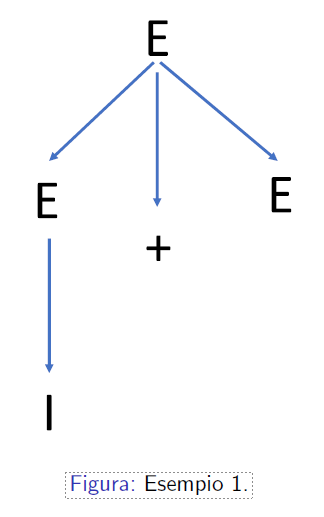
\includegraphics[width=3cm]{./Images/2.1.png}
\end{figure}
\FloatBarrier

Esempio $2 .$

Un albero sintattico per la grammatica delle parole palindrome binarie $G_{p a l}=(\{S\},\{0,1\}, P, S)$ e
$$
P=\{S \rightarrow \epsilon|0| 1|0 S 0| 1 S 1\}
$$


\begin{figure}[hbpt!]
    \centering
    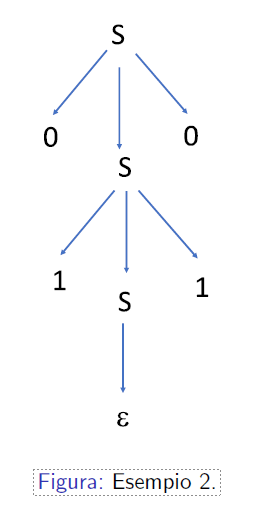
\includegraphics[width=3cm]{./Images/2.2.png}
\end{figure}
\FloatBarrier

\subsubsection{Prodotto di un albero sintattico}
Il prodotto (o frontiera) di un albero sintattico è la parola che si ottiene concatenando le etichette delle foglie a partire da sinistra.ù

- Di particolare importanza sono gli alberi sintattici che soddisfano le due seguenti condizioni.
\begin{enumerate}
    \item Il prodotto è una stringa sull'alfabeto dei terminali, cioè ogni foglia ha come etichetta un terminale o $\epsilon$.
    \item La radice ha come etichetta il simbolo iniziale.
\end{enumerate}
Questi alberi sono importanti perché vedremo che una parola è nel linguaggio di una grammatica se e solo se è il prodotto di un albero di questo tipo.

\vspace{5mm}

Esempio 3

Un albero sintattico per la grammatica $G_{E}=(\{E, I\}, T, P, E)$ per espressioni aritmetiche dove
$$
T=\{+, *,(,), a, b, 0,1\}
$$
e
$$
\begin{aligned}
P=&\{E \rightarrow E+E|E * E|(E) \mid I\\
&I \rightarrow a|b| Ia| Ib| I0 | I1\}
\end{aligned}
$$
II prodotto $a *(a+b 00)$ è una stringa sull'alfabeto dei terminali. La radice ha come etichetta il simbolo iniziale della grammatica.

\begin{figure}[hbpt!]
    \centering
    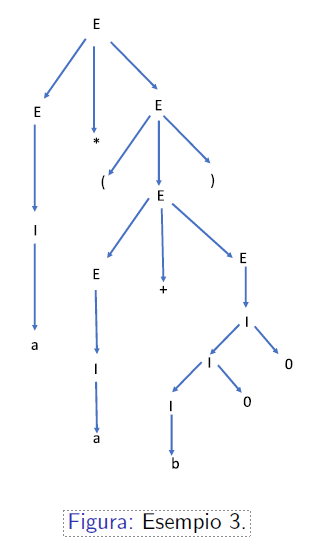
\includegraphics[width=4cm]{./Images/2.3.png}
\end{figure}
\FloatBarrier

Esempio 3

Abbiamo mostrato una derivazione della stringa $a *(a+b 00)$ in $G_{E}$.
$$
\begin{aligned}
&E \Rightarrow E * E \Rightarrow I * E \Rightarrow a * E \Rightarrow a *(E) \Rightarrow \\
&a *(E+E) \Rightarrow a *(I+E) \Rightarrow a *(a+E) \Rightarrow a *(a+I) \Rightarrow \\
&a *(a+I 0) \Rightarrow a *(a+100) \Rightarrow a *(a+b 00)
\end{aligned}
$$
Vedremo che questo particolare parse tree è una rappresentazione della derivazione.

\subsubsection{Alberi sintattici e derivazioni}

Teorema

Sia $G=(V, T, P, S)$ una grammatica context free, sia $A \in V e$ $w \in T^{*}$. Le condizioni seguenti sono equivalenti.
\begin{enumerate}
    \item Esiste un albero sintattico con radice etichettata da $A$ e con prodotto $w$
    \item $A \xRightarrow[lm]{*} w$
    \item $A \xRightarrow[rm]{*} w$
    \item $A \xRightarrow[]{*} w$
\end{enumerate}

Proveremo che (1) implica (2)
e che (1) implica (3)
Poi che (4) implica (1).
La dimostrazione `e terminata. Infatti poiché è evidente che (2) implica (4), avremo provato che le condizioni (1), (2), (4) sono equivalenti.
Analogamente, poiché è evidente che (3) implica (4), avremo provato che le condizioni (1), (3), (4) sono equivalenti.
Quindi le quattro condizioni sono equivalenti.

Nelle dimostrazioni vengono utilizzati due risultati intermedi.
Ricordiamo la definizione di derivazione diretta: se $A \rightarrow \gamma$ è una produzione in $G$ allora $\alpha A \beta \xRightarrow[G]{} \gamma \beta$, per ogni $\alpha, \gamma, \operatorname{con} \alpha, \gamma$ stringhe di variabili e terminali.
Il primo risultato che si utilizza è una estensione di tale definizione: Se $A \xRightarrow[]{*} \gamma$, questa derivazione si può inserire in un contesto, cioè $\alpha A \beta \xRightarrow[]{*} \alpha \gamma \beta$. Con un ipotesi aggiuntiva su $\alpha$ (risp. $\beta$) lo stesso risultato vale per le derivazioni a sinistra (risp. a destra).
Chiameremo questa proprietà la proprietà dell'inserzione.

\subsubsection{Proprietà dell'inserzione}

Sia $G=(V, T, P, S)$ una grammatica context free. Per ogni $A \in V \cup T, \alpha, \gamma_{1}, \gamma_{2} \in(V \cup T)^{*}$,
\begin{itemize}
    \item se $A \xRightarrow[G]{*} \alpha$ allora $\gamma_{1} A \gamma_{2} \xRightarrow[G]{*} \gamma_{1} \alpha \gamma_{2}$
    \item se $A \xRightarrow[lm]{*} \alpha \alpha \mathrm{e} \gamma_{1} \in T^{*}$ allora $\gamma_{1} A \gamma_{2} \xRightarrow[lm]{*} \gamma_{1} \alpha \gamma_{2}$
    \item se $A \xRightarrow[rm]{*} \alpha e \gamma_{2} \in T^{*}$ allora $\gamma_{1} A \gamma_{2} \xRightarrow[rm]{*} \gamma_{1} \alpha \gamma_{2}$
\end{itemize}

Teorema

Sia $G=(V, T, P, S)$ una grammatica context free.
Se esiste un albero sintattico con radice etichettata da una variabile $A$ e con prodotto $w$, dove $w \in T^{*}$, allora esiste una derivazione a sinistra $A \xRightarrow[lm]{*} w$ nella grammatica $G$.

\vspace{5mm}

(Dall'albero sintattico alla derivazione a sinistra)
La prova è per induzione strutturale sull'altezza dell'albero.

\textbf{Passo Base.} L'altezza minima che può avere un albero sintattico con radice in $V$ e un prodotto che sia una stringa di terminali è $1 .$

Se $\mathcal{T}$ è un albero sintattico di altezza 1 , con radice etichettata da una variabile $A$ e con prodotto $w$, dove $w \in T^{*}$, allora l'albero è formato dalla radice $A$ che ha come figli, da sinistra, etichettati $X_{1}, X_{2}, \ldots, X_{k}$ e $X_{1} X_{2} \cdots X_{k}=w$.
Per definizione di albero sintattico, $A \rightarrow X_{1} X_{2} \cdots X_{k}$ è una produzione in $G$ e quindi $A \stackrel{*}{\Rightarrow} X_{1} X_{2} \cdots X_{k}=w$ nella grammatica $G$.

\begin{figure}[hbpt!]
    \centering
    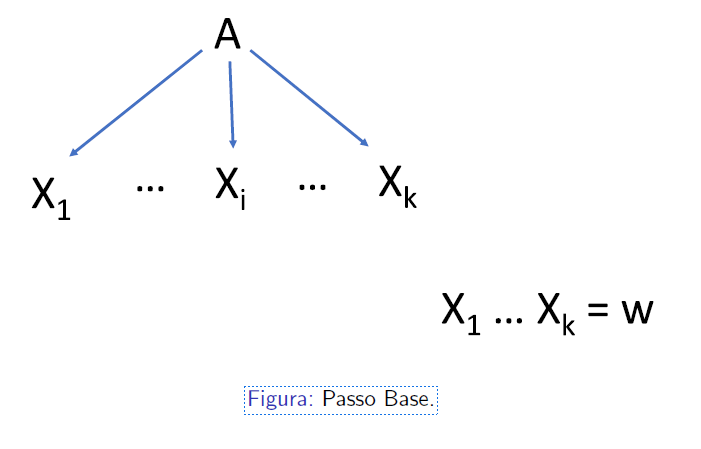
\includegraphics[width=6cm]{./Images/2.4.png}
\end{figure}
\FloatBarrier

(Dall'albero sintattico alla derivazione a sinistra)
\textbf{Passo Ricorsivo.} Sia $\mathcal{T}$ un albero sintattico di altezza $n>1$, con radice etichettata da una variabile $A$ e con prodotto $w$, dove $w \in T^{*}$. La radice avrà figli, da sinistra, etichettati $X_{1}, X_{2}, \ldots, X_{k}$, con $X_{1}, X_{2}, \ldots, X_{k} \in V \cup T$.
Se $X_{i} \in T$, poniamo $X_{i}=w_{i}$. Se $X_{i} \in V$ allora $X_{i}$ è la radice di un sottoalbero $\mathcal{T}_{i}$ di $\mathcal{T}$ di altezza $n-1 \geq 1$. Chiamiamo $w_{i}$ il prodotto di $\mathcal{T}_{i}$.
Osserviamo che $w_{1} w_{2} \cdots w_{k}=w$


\begin{figure}[hbpt!]
    \centering
    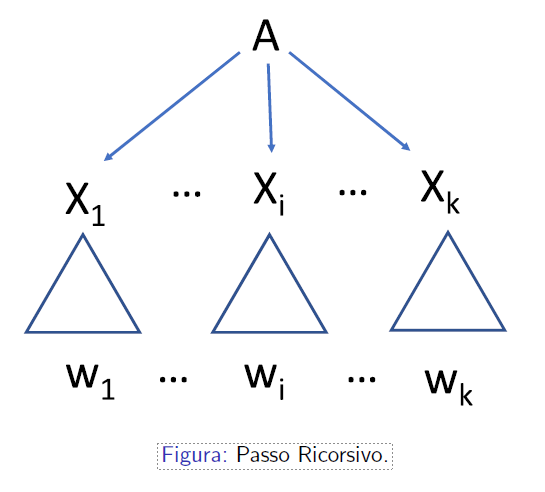
\includegraphics[width=5cm]{./Images/2.5.png}
\end{figure}
\FloatBarrier

(Dall'albero sintattico alla derivazione a sinistra)
\textbf{Passo Ricorsivo.} Sia $\mathcal{T}$ un albero sintattico di altezza $n>1$, con radice etichettata da una variabile $A$ e con prodotto $w$, dove $w \in T^{*}$. La radice avrà figli, da sinistra, etichettati $X_{1}, X_{2}, \ldots, X_{k}, \operatorname{con} X_{1}, X_{2}, \ldots, X_{k} \in V \cup T$
Se $X_{i} \in T$, poniamo $X_{i}=w_{i} .$ Se $X_{i} \in V$ allora $X_{i}$ è la radice di un sottoalbero $\mathcal{T}_{i}$ di $\mathcal{T}$ di altezza $n-1 \geq 1$. Chiamiamo $w_{i}$ il prodotto di $\mathcal{T}_{i}$.
Osserviamo che:
(1) $A \xRightarrow[lm]{*} X_{1} X_{2} \cdots X_{k}$ (per definizione di albero sintattico)
(2) $X_{i} \xRightarrow[lm]{*} w_{i}$ (per ipotesi induttiva)
(3) $w_{1} w_{2} \cdots w_{k}=w$

\vspace{5mm}

Proviamo, per induzione su $i$, che per $i=0, \ldots, k$,
$$
A \xRightarrow[lm]{*} w_{1} w_{2} \cdots w_{i} X_{i+1} X_{i+2} \cdots X_{k}
$$
Passo Base. $i=0$ e sappiamo che $A \xRightarrow[lm]{*} X_{1} X_{2} \cdots X_{k}$.
Passo Induttivo. Supponiamo che
$$
A \xRightarrow[lm]{*} w_{1} w_{2} \cdots w_{i-1} x_{i} x_{i+2} \cdots x_{k}
$$
Se $X_{i}=w_{i}$, allora
$$
A \xRightarrow[lm]{*} w_{1} w_{2} \cdots w_{i} X_{i+1} X_{i+2} \cdots X_{k}
$$
Altrimenti $X_{i} \xRightarrow[lm]{*} w_{i}$ e grazie alla proprietà dell'inserzione
$$
A \xRightarrow[lm]{*} w_{1} w_{2} \cdots w_{i} X_{i+1} X_{i+2} \cdots X_{k}
$$
Per $i=k$ otteniamo
$$
A \xRightarrow[lm]{*} w_{1} w_{2} \cdots w_{k}=w
$$

\vspace{5mm}

Teorema

Sia $G=(V, T, P, S)$ una grammatica context free.

Se esiste un albero sintattico con radice etichettata da una variabile $A$ e con prodotto $w$, dove $w \in T^{*}$, allora esiste una derivazione a destra $A \underset{r m}{\stackrel{*}{\Rightarrow}} w$ nella grammatica $G$.
La dimostrazione di questo teorema è molto simile alla precedente.

\subsubsection{Proprietà della fattorizzazione}

Adesso vogliamo provare un enunciato che è quasi l'inverso: se esiste una derivazione $A \underset{}{\stackrel{*}{\Rightarrow}} w$ nella grammatica $G$, dove $A \in V$ e $w \in T^{*}$, allora $w$ è il prodotto di un albero sintattico con radice etichettata $A$.

Ci serve una seconda proprietà delle grammatiche context-free. Questa proprietà afferma che se una stringa $\alpha$ di variabili e terminali può essere derivata da $X_{1} X_{2} \cdots X_{n}$, dove ogni $X_{i}$ è una variabile o un terminale, esiste una fattorizzazione $\alpha=\alpha_{1} \alpha_{2} \cdots \alpha_{n}$ di $\alpha$ tale che ogni $X_{i}$ deriva la corrispondente stringa $\alpha_{i}$.

Chiameremo questa proprietà la proprietà della fattorizzazione.

Sia $G=(V, T, P, S)$ una grammatica context free. Se
$$
X_{1} X_{2} \cdots X_{n} \underset{G}{\stackrel{*}{\Rightarrow}} \alpha
$$
$\operatorname{con} X_{1}, X_{2}, \ldots, X_{n} \in V \cup T, n \geq 1, \alpha \in(V \cup T)^{*}$, allora esistono $\alpha_{1}, \alpha_{2}, \ldots, \alpha_{n} \in(V \cup T)^{*}$ tali che
(1) $\alpha=\alpha_{1} \alpha_{2} \cdots \alpha_{n}$
(2) $X_{i} \underset{G}{\stackrel{*}{\Rightarrow}} \alpha_{i}$, per $i=1,2, \ldots, n$
(3) Il numero dei passi (numero di derivazioni dirette) in $X_{1} X_{2} \cdots X_{n} \underset{G}{\stackrel{*}{\Rightarrow}} \alpha$ è la somma del numero dei passi in $X_{i} \underset{G}{\stackrel{*}{\Rightarrow}} \alpha_{i}$, per $i=1,2, \ldots, n$
(4) Se $X_{i} \in T$ allora $X_{i}=\alpha_{i}$.

\vspace{5mm}

Teorema

Sia $G=(V, T, P, S)$ una grammatica context free.

Se esiste una derivazione $A \neq w$ nella grammatica $G$, dove $A \in V$ e $w \in T^{*}$, allora esiste un albero sintattico con radice etichettata A e con prodotto $w$.

\subsubsection{Grammatiche ambigue}

Una grammatica context-free $G=(V, T, P, S)$ è ambigua se esiste almeno una stringa $w$ in $T^{*}$ per la quale possiamo trovare due alberi sintattici distinti, ciascuno con radice etichettata $S$ e con prodotto $w$.

\vspace{5mm}

- Nota. $G=(V, T, P, S)$ è non ambigua se per ogni $w$ in $T^{*}$ possiamo trovare al più un albero sintattico con radice etichettata $S$ e con prodotto $w$.

La figura seguente mostra due alberi sintattici distinti della grammatica $G_{E}=(\{E, I\}, T, P, E)$ per espressioni aritmetiche che hanno come prodotto $I+I * I$.

\begin{figure}[hbpt!]
    \centering
    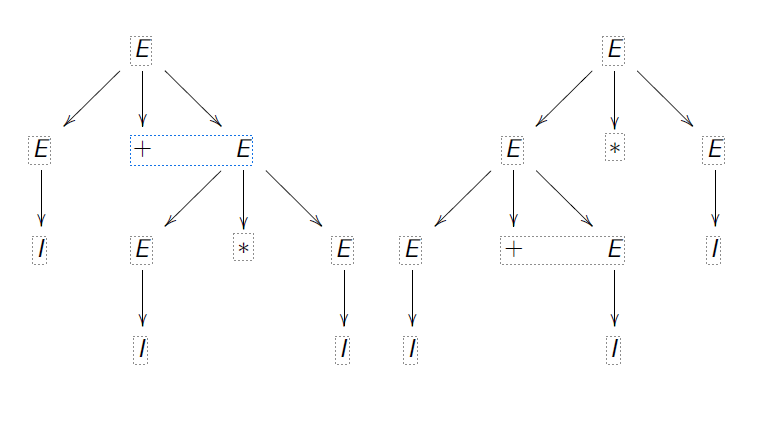
\includegraphics[width=6cm]{./Images/2.6.png}
\end{figure}
\FloatBarrier

Possiamo facilmente ricavare dai due alberi precedenti due alberi sintattici distinti di $G_{E}$ con prodotto una stringa di terminali, ad esempio $a+a * a$, e quindi $G_{E}$ è ambigua.
\begin{figure}[hbpt!]
    \centering
    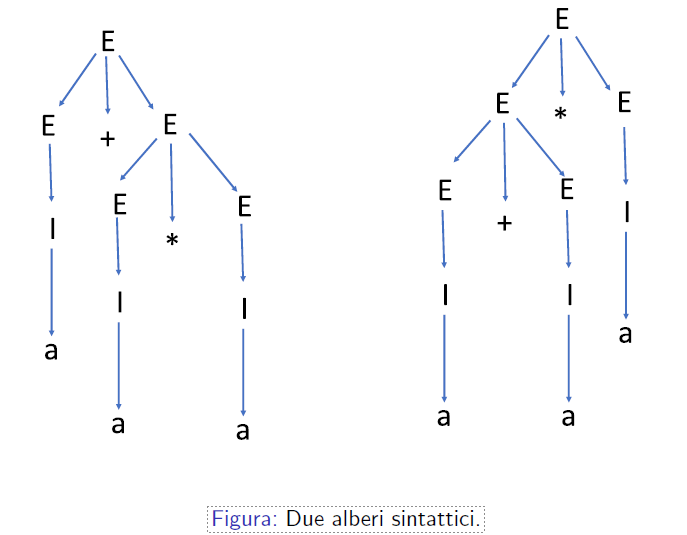
\includegraphics[width=6cm]{./Images/2.7.png}
\end{figure}
\FloatBarrier

Nota. 

$G=(V, T, P, S)$ è non ambigua se per ogni $w$ in $T^{*}$ possiamo trovare al più un albero sintattico con radice etichettata $S$ e con prodotto $w$.

Gli alberi sintattici permettono di associare una struttura a un programma. Se questa struttura non è unica questo diventa un problema.

Siccome gli alberi sintattici sono legati alle derivazioni si potrebbe sospettare che l'esistenza di più alberi sintattici di una grammatica con lo stesso prodotto dipenda dal numero di possibili derivazioni di una stringa.

- Nota. L'ambiguità di $G$ non dipende dal fatto che una stringa ammette due derivazioni distinte poiché esse possono dar luogo allo stesso albero sintattico.

- Esempio. In $G_{E}$ le due seguenti derivazioni danno luogo allo stesso albero sintattico.
$$
\begin{aligned}
E & \Rightarrow E+E \Rightarrow I+E \Rightarrow a+E \Rightarrow a+I \Rightarrow a+b \\
E & \Rightarrow E+E \Rightarrow E+I \Rightarrow I+I \Rightarrow I+b \Rightarrow a+b
\end{aligned}
$$

\begin{figure}[hbpt!]
    \centering
    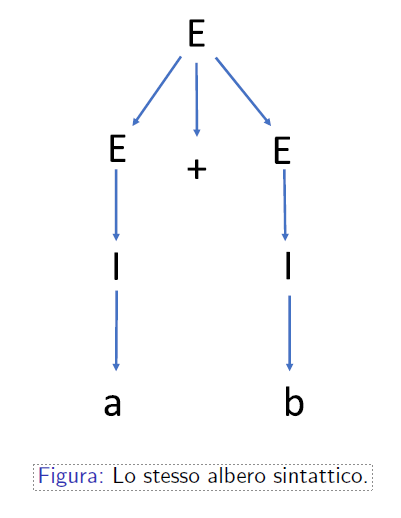
\includegraphics[width=4cm]{./Images/2.8.png}
\end{figure}
\FloatBarrier

\subsubsection{Derivazioni a sinistra e ambiguità}

Teorema
Per ogni CFG $ G=(V, T, P, S)$ e per ogni $w \in T^{*}$, la stringa $w$ ha due alberi sintattici distinti, con radice etichettata $S$ e con prodotto $w$, se e solo se $w$ ha due distinte derivazioni sinistre da S.


- Nota. Quindi una grammatica context-free $G=(V, T, P, S)$ è ambigua se esiste almeno una stringa $w$ in $T^{*}$ che ha due distinte derivazioni sinistre da $S$.

\subsubsection{Eliminare le ambiguità da una grammatica}

Due grammatiche context-free $G, G^{\prime}$ sono equivalenti se $L(G)=L\left(G^{\prime}\right)$

- Nota. Data una grammatica context-free ambigua $G$, a volte è possibile trasformarla in una grammatica context-free $G^{\prime}$, dove $G^{\prime}$ è equivalente a $G$ e $G^{\prime}$ è non ambigua.

Nota. E possibile ad esempio trasformare $G_{E}$ in una grammatica context-free $G^{\prime}$, dove $G^{\prime}$ è equivalente a $G_{E}$ e $G^{\prime}$ è non ambigua.

Una grammatica non ambigua che genera lo stesso linguaggio di $G_{E}$ è $G_{E}^{\prime}=\left(V^{\prime}, \Sigma, P^{\prime}, E\right)$, dove $V^{\prime}=\{E, F, T, I\}$, $\Sigma=\{a, b, 0,1,(,),+, *$,$ e P^{\prime}$ consiste delle produzioni
$$
\begin{aligned}
I & \rightarrow a|b| Ia|Ib|I0|I1 \\
F & \rightarrow I \mid(E) \\
T & \rightarrow F \mid T * F \\
E & \rightarrow T \mid E+T
\end{aligned}
$$

- Esiste un algoritmo per decidere se una CFG è ambigua?
No
$$
L=\{\langle G\rangle \mid G \text { è una CFGe Gè ambigua }\}
$$
è indecidibile.
- Esiste un algoritmo per trasformare una CFG ambigua in una CFG equivalente e non ambigua?
No

- È sempre possibile trasformare una CFG ambigua in una CFG equivalente e non ambigua?
No.

Esistono CFG G ambigue e tali che ogni grammatica equivalente a $G$ è ambigua.
In tal caso $L(G)$ si dice inerentemente ambiguo.

\subsubsection{Ambiguità inerente}

Un linguaggio context-free $L$ è inerentemente ambiguo se ogni grammatica che lo genera è ambigua.
\begin{itemize}
    \item Un CFL L non è inerentemente ambiguo se esiste una CFG non ambigua $G$ tale che $L=L(G)$.
    \item Il linguaggio $L\left(G_{E}\right)$ delle espressioni aritmetiche non è inerentemente ambiguo.
    \item Vedremo che i linguaggi regolari sono linguaggi context-free non inerentemente ambigui.
    \item Un linguaggio inerentemente ambiguo:
$$
L=\left\{a^{n} b^{m} c^{m} d^{n} \mid n \geq 1, m \geq 1\right\} \cup\left\{a^{n} b^{n} c^{m} d^{m} \mid n \geq 1, m \geq 1\right\}
$$
è inerentemente ambiguo ed è generato dalla seguente grammatica context-free
$$
S \rightarrow A \mid C D
$$
$A \rightarrow a A d|a B d \quad B \rightarrow b B c| b c \quad C \rightarrow a C b|a b \quad D \rightarrow c D d| c d$
Esercizio: provare a generare la stringa aabbccdd con le due derivazioni canoniche sinistre che iniziano con le due produzioni per $S$.
\end{itemize}

\let\cleardoublepage\clearpage
\subsubsection{}
% \xRightarrow[G]{*}
% \underset{r m}{\stackrel{*}{\Rightarrow}}